\documentclass{article}

\usepackage[french]{babel} % langue
\usepackage[utf8]{inputenc}
\usepackage[T1]{fontenc}
\usepackage{xspace} % espacement
\usepackage{physics} % dérivées
\usepackage{amssymb}
\usepackage{graphicx}

\usepackage{siunitx}
\sisetup{
    detect-all,
    output-decimal-marker={,},
    group-minimum-digits = 3,
    group-separator={~},
    number-unit-separator={~},
    inter-unit-product={~}
}
\newcommand{\cel}{\degreeCelsius}

\usepackage{pythonhighlight} % coloration
\definecolor{keywordcolour}{HTML}{5e81ac}
\definecolor{literatecolour}{HTML}{5e81ac}
\definecolor{stringcolour}{HTML}{008000}
\usepackage{listingsutf8}
\lstset{
    basicstyle=\small\ttfamily,
    columns=flexible,
    breaklines=true
}

\usepackage{tikz}
\definecolor{nord10}{RGB}{94,129,172}
\definecolor{nord11}{RGB}{191,97,106}

\newcommand{\p}{\texttt} % Stylisé comme du code.
\newcommand{\air}{$\Lambda$\xspace}
\newcommand{\cair}{C_{\Lambda}}
\newcommand{\tair}{T_{air}}
\newcommand{\ordi}{$\Sigma$\xspace}
\newcommand{\etdt}{entre $t$ et $t + \dd t$\xspace}
\newcommand{\exdx}{entre $x$ et $x + \dd x$\xspace}

\usepackage{graphicx}
\graphicspath{ {./images/} }

\title{Simulation : cahier des charges}
\author{Malo Leroy -- Ulysse Tanguy--Bompard}

\begin{document}

\maketitle

\section{Objectifs}

On cherche à réaliser une simulation des échanges thermiques entre deux systèmes :
\begin{itemize}
    \item Un ordinateur (\ordi), recevant  une puissance $P$, initialement à la température $T_0$
    \item Le milieu extérieur (\air), qu'on considèrera être de l'air (sec)
\end{itemize}

On supposera dans un premier temps que le système \air est un thermostat à la température $T_0$ (hypothèse A). Dans un second temps on considèrera que \{\ordi + $\Lambda$\} est un système isolé (hypothèse B).

\section{Constantes thermodynamiques}

\subsection{Ordinateur}

On considère que l'ordinateur a une masse $m$ et une capacité thermique massique $c$ uniforme, d'où une capacité thermique $C = c m$. Sa conductivité thermique est notée $\lambda$. Sa masse volumique (moyenne), supposée uniforme, est notée $\rho$. La diffusivité thermique est alors $D = \frac{\lambda} {\rho c}$.

Le processeur a une capacité thermique $C_p$, ainsi la capacité thermique de la carcasse est $C - C_p$.

\subsection{Air}

On notera les constantes thermodynamiques relatives à l'air avec un indice $a$. On prend pour conductivité thermique de l'air à pression consante $P = \SI{1}{bar}$, avec $T$ la température de l'air exprimée en degrés celsius \footnote{Voir  WG Kannuluik and EH Carman, \textit{The Temperature Dependence of the Thermal Conductivity of Air}, DOI CH9510305} et $\lambda_{a}$ en $\SI{}{mW.m^{-1}.K^{-1}}$

$$\lambda_{a} = -0.000044075614398888 \times T^2 + 0.0766069577308689*T + 24.3560822452597$$

\begin{python}
def lambda_air(T): # W.m^-1.K^-1, a 1 bar
    vA = celsius(T)
    l = -0.000044075614398888*vA*vA+0.0766069577308689*vA+24.3560822452597
    return l / 1000
\end{python}

La loi des gaz parfaits donne pour l'air, lorsque $T$ est exprimé en kelvins

$$\rho_a = \frac{PM}{RT} = \frac{346384}{T}$$

\begin{python}
def rho_a(T):
    return 346384 / T
\end{python}

Cela permet de définir la diffusivité de l'air $D_a = \frac{\lambda_a}{\rho_a c_a}$

\section{Calculs généraux}

L'équation de la chaleur obtenue est, au point $M$ de l'espace et à l'instant $t$

$$\rho(M) c(M) \pdv{T}{t}\/(M, t) = \lambda (M) \Delta T(M, t) $$

\section{Modélisations}

\subsection{Modèle unidimentionnel}

On considère que l'espace de travail est un axe $(Ox)$, en fait un cylindre de section $S$ et de longueur $l_a = \SI{1}{m}$, et que l'ordinateur est représenté par un segment de longueur $l = \SI{10}{cm}$ (toutes les grandeurs ne dépendent de $y$ ou $z$). On considère que la source de puissance est un segment de longueur $l_p = \SI{1}{cm}$ centré par rapport au segment de longueur $l$.

\begin{tikzpicture}
    \draw[thick] (0, 0) -- (9, 0) node [above, sloped] {$l_a$};
    \draw[purple, ultra thick] (2, 0) -- (7, 0) node [above, sloped] {$l$};
    \draw[blue, ultra thick] (4, 0) -- (5, 0) node [midway, above, sloped] {$l_p$};
\end{tikzpicture}

La température dépend de l'espace via la variable $x$ et du temps via la variable $t$, ainsi on la représente par la fonction notée $T(x, t)$, ou par la matrice \p{T[i][j]}, où \p{i} et \p{j} sont des entiers lorsque l'espace et le temps sont discrétisés.

L'équation bien connue obtenue est, en faisant apparaître les dépendances aux variables $x$ et $t$
$$\rho(x) c(x) \pdv{T}{t} = \pdv{x} \left( \lambda (x) \pdv{T}{x} \right) + P_v(x)$$
Les fonctions $\rho$, $c$ et $\lambda$ étant des fonctions en escalier (toutes de mêmes paliers), on peut raisonnablement écrire

$$\pdv{T}{t} = D(x) \pdv[2]{T}{x} + P_c$$

où $P_c = P_v / (\rho c)$ s'exprime en $\SI{}{K.s^{-1}}$. Détaillons la valeur de $D(x)$ et celle de $P_c(x)$ dans chacun des trois milieux.
\begin{itemize}
    \item Source : $D(x) = D$ et $P_c(x) = P / C_p$ où $C_p = l_p S \rho c$
    \item Carcasse : $D(x) = D$ et $P_c(x) = 0$
    \item Air : $D(x) = D_a$ et $P_c(x) = 0$
\end{itemize}

Dans un modèle discret où le pas de temps est $t_e$ et le pas d'espace est $x_e$,  cette équation se réécrit
$$T(x, t+t_e) = T(x, t) + \frac{t_e}{{x_e}^2} D(x)
    \left( T(x+x_e, t) - T(x, t) + T(x-x_e, t) \right)
    + P_c(x) t_e$$

\begin{python}
T[xi, ti+1] = T[xi, ti] + (t_e / (x_e**2)) * D(xi)
    (T[xi+1, ti] - T[xi, ti] + T[xi-1, ti])
    + P_c(xi) * t_e
\end{python}

\subsubsection{Hypothèse A}

Puisque les bords extérieurs de l'ordinateur sont à la même température que l'air, on se limite à l'étude d'un espace de longueur $l$ : les positions s'étalent entre $x = 0$ et $x = l$.

L'hypothèse A se traduit ainsi par les conditions aux limites $\forall t,~T(x=0, t) = T(x=l, t) = T_0$, c'est-à-dire $\forall$ \p{ti}, \p{T[0, ti] = T[-1, ti] = T0}.

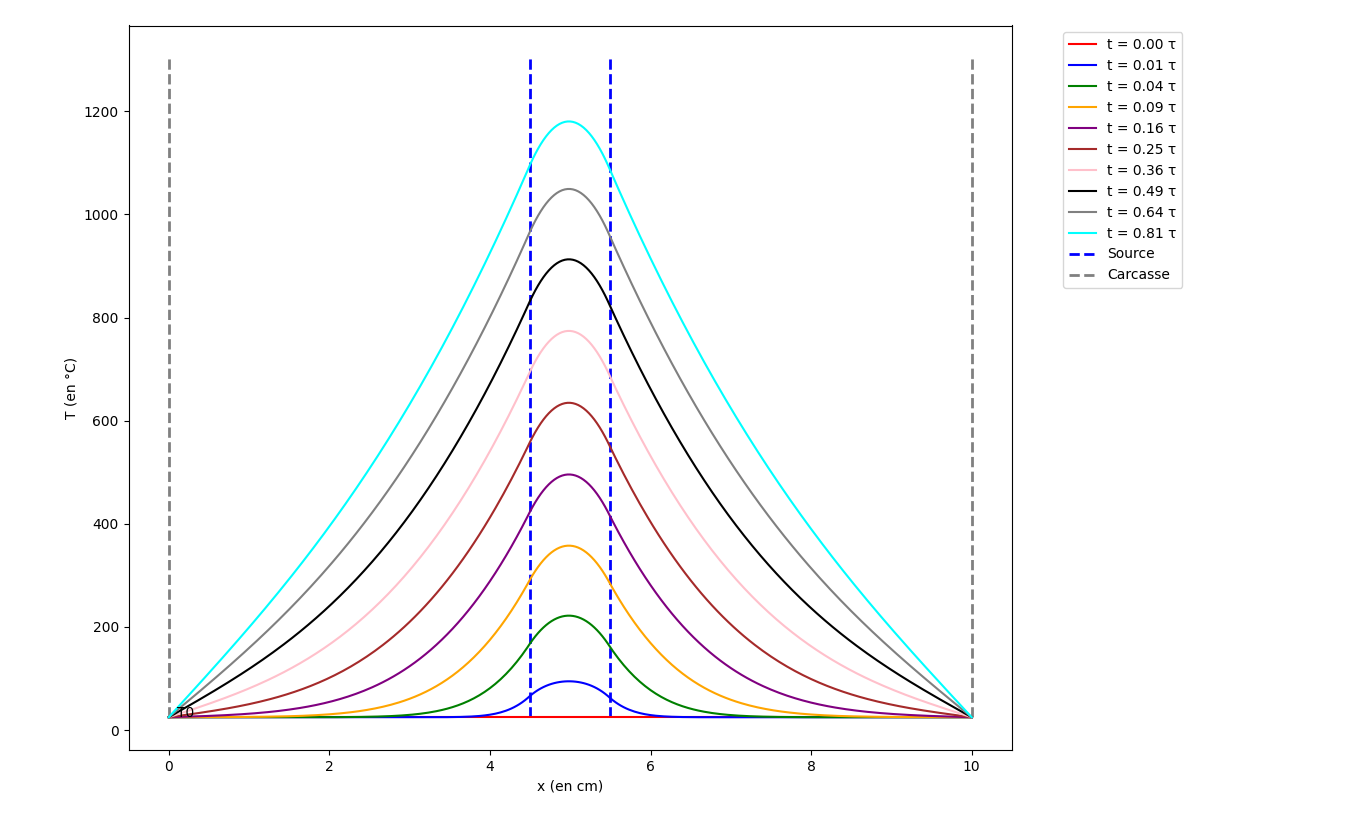
\includegraphics[scale=0.37]{1dA_P500mW_t11s.png}

Ci-dessus se trouve une visualisation des résultats sous l'hypothèse d'une puissance constante $P = \SI{500}{mW}$. Le temps d'échelle vaut $\tau = \SI{11}{s}$. La figure ci-dessous montre pour un temps $\tau = \SI{2}{min}$ les résultats obtenus en régime permanent.

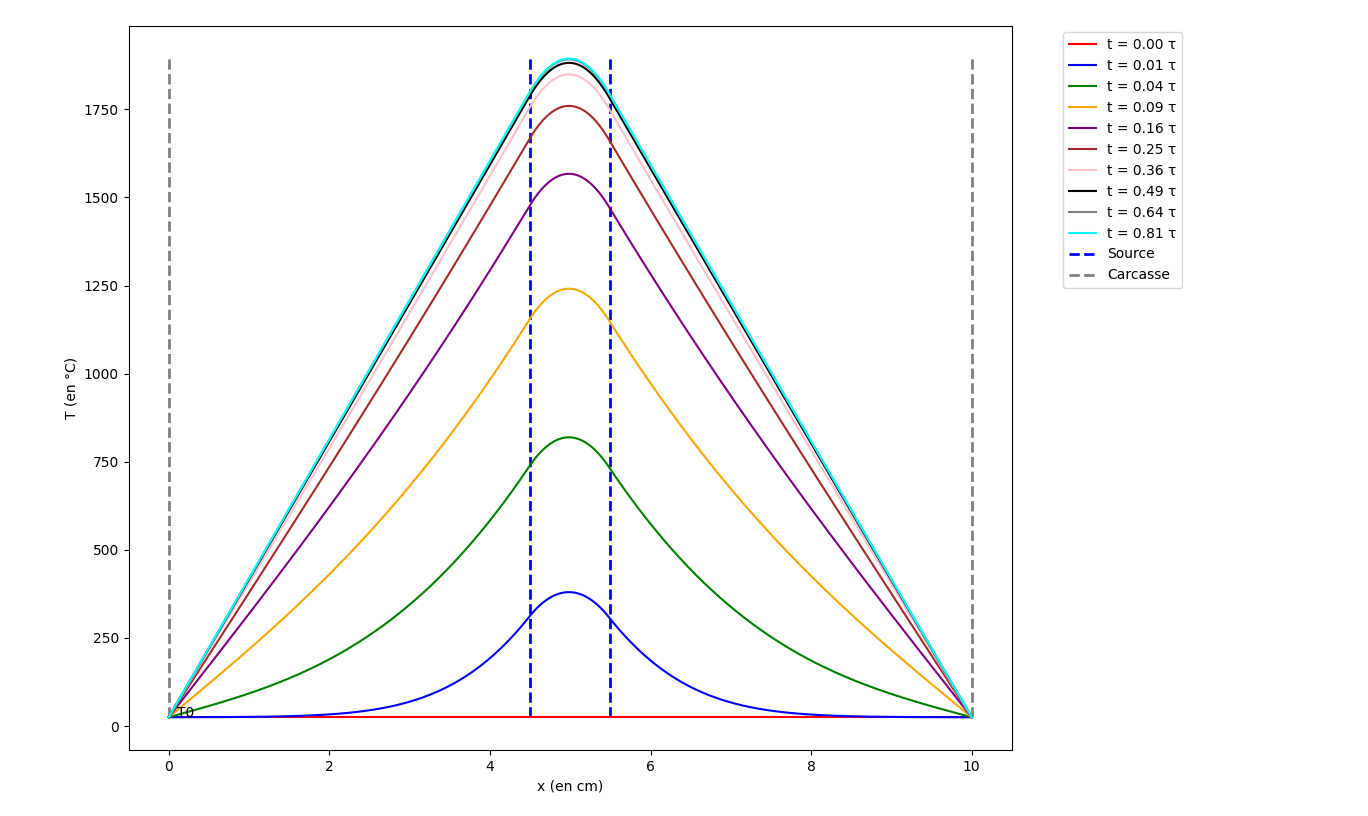
\includegraphics[scale=0.37]{1dA_P500mW_t110s.png}

\subsubsection{Hypothèse B}

On considère plus, dans le cadre de cette hypothèse que l'espace d'observation est limité à l'ordinateur : celui-ci est entouré d'air. L'extension totale de l'espace est alors de $l_a$ (air et ordinateur compris).

La condition aux limites est cette fois dynamique : on impose une « continuité » de la température aux extrémités de l'espace. Physiquement, cela correspond à un modèle où le système (air compris) est placé dans une enceinte parfaitement calorifugée. Pour tout \p{ti} tel que \p{T[:, ti]} ait déjà été calculé, on impose alors \p{T[0, ti+1] = T[1, ti+1]} et \p{T[-1, ti+1] = T[-2, ti+1]}.

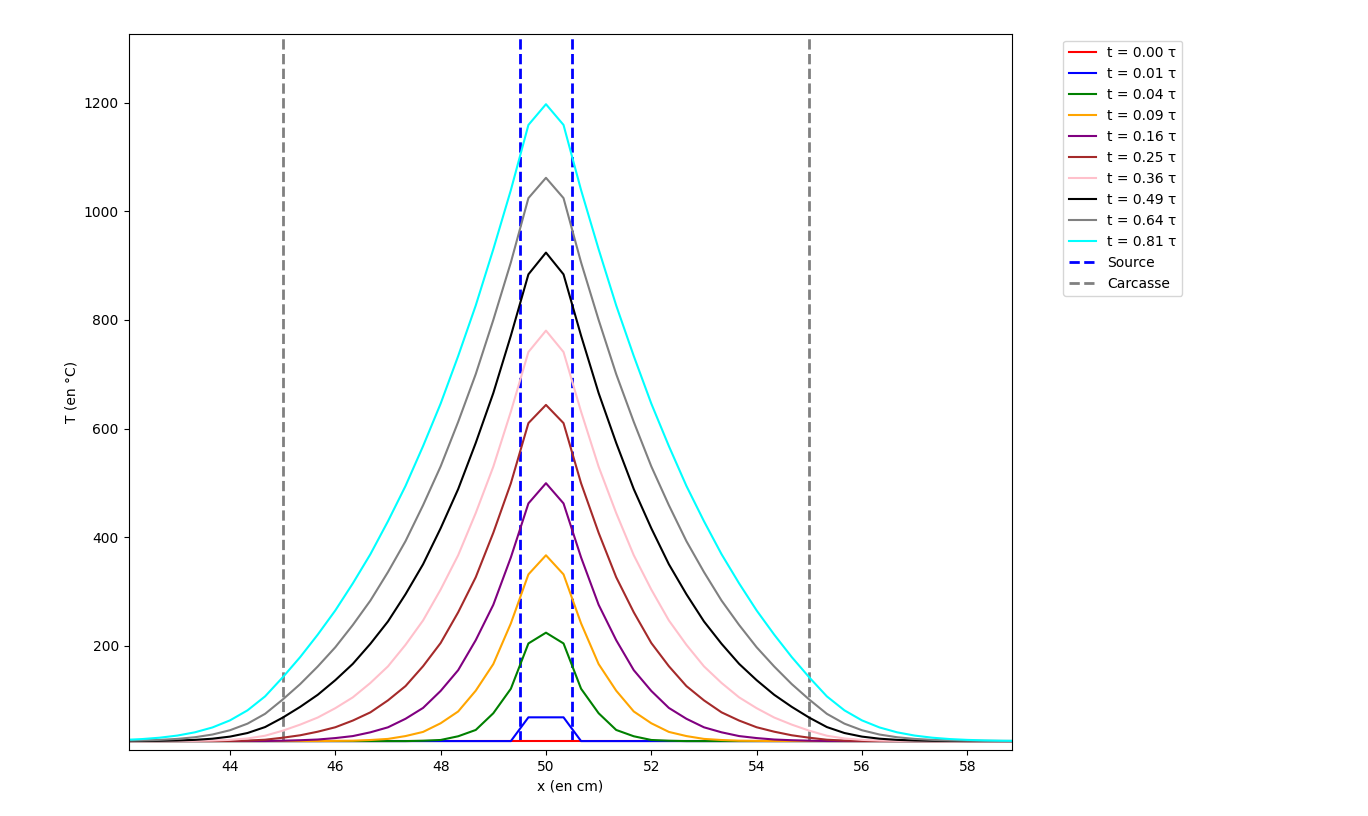
\includegraphics[scale=0.37]{1dB_P500mW_t11s.png}

Ci-dessus se trouve une visualisation des résultats sous l'hypothèse d'une puissance constante $P = \SI{500}{mW}$. Pour $\tau = \SI{11}{s}$, on a un résultat équivalent à celui obtenu dans le cadre de l'hypothèse A en raison de la faible valeur de $\tau$. Ce n'est plus le cas pour des temps d'échelle plus grands, ci-dessus avec $\tau = \SI{3}{h}$, qui permettent d'observer le comportement du système en régime permanent.

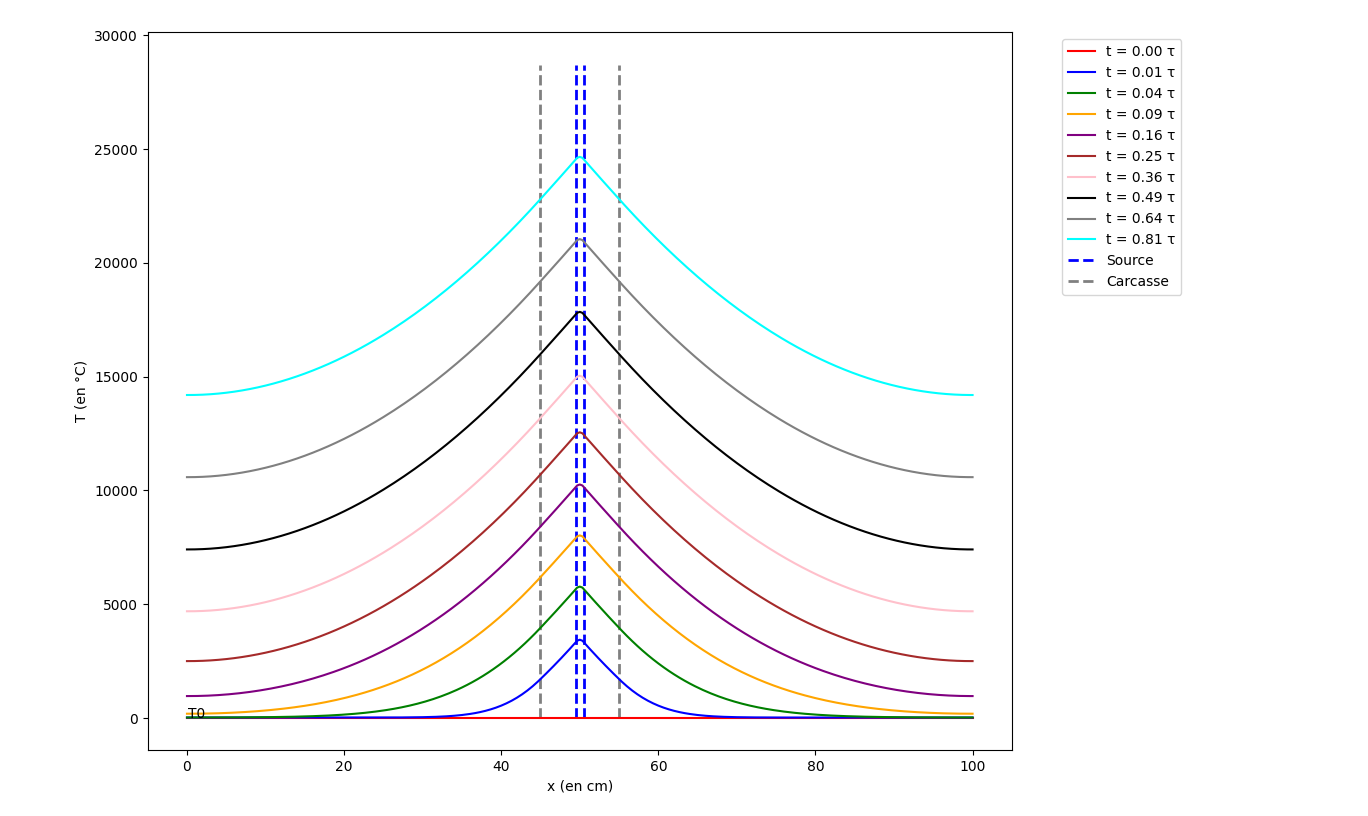
\includegraphics[scale=0.37]{1dB_P500mW_t11000s.png}


\subsection{Modèle bidimensionnel}

L'espace est un plan $(Oxy)$, fini et d'extension totale un carré de côté $l_a = \SI{1}{m}$, si besoin considéré d'épaisseur $e = \SI{1}{cm}$, mais les grandeurs en jeu ne dépendent spatialement que de $x$ et $y$. L'ordinateur est représenté par un carré de côté $l = \SI{10}{cm}$, et le processeur par un carré de côté $l_p = \SI{1}{cm}$ centré sur le reste de l'ordinateur.

\begin{tikzpicture}[scale=0.50]
    \draw (0, 0) rectangle (9, 9);
    \fill[nord10] (2, 2) rectangle (7, 7);
    \fill[nord11] (4, 4) rectangle (5, 5);
    \node at (10, 8) {$l_a$};
    \node[nord10] at (8, 7) {$l$};
    \node[nord11] at (6, 6) {$l_p$};
\end{tikzpicture}

L'équation obtenue est, par le même travail que précédemment

$$\pdv{T}{t} = D(x, y) \left( \pdv[2]{T}{x} + \pdv[2]{T}{y} \right)+ P_c$$

\section*{Annexe : notations}

\begin{itemize}
    \item Un nom de variable, un nom de fonction, n'a pas de majuscule. On ne peut pas nommer une variable ou une fonction \p{lambda}.
    \item Si on a besoin de donner un nom long à une variable, ou à une fonction, on met des « \_ » par exemple \p{grande\_chaise\_rouge}
    \item Il n'y a pas d'espace autour de parenthèses lors d'un appel ou d'une définition de fonction
    \item Autour d'un égal de définition (\p{=}) ou d'un signe de relation (\p{==}, \p{<=}, \p{<}, etc.) il y a des espaces, un avant et un après
    \item Dans du code comme dans un \LaTeX, après une virgule il y a un espace
\end{itemize}

\end{document}
